\chapter{2023}
\section*{一. 程序阅读题(本大题共 4 小题,共 20 分)}

1. (4 分) 有一段代码:
\begin{lstlisting}[language=C, basicstyle=\ttfamily]
int brute(int a[], int N) {
    int i,j,k,m;
    for(i=0;i<N;i++)
        for(j=i+1;j<N;j++)
            for(k=j+1;k<N;k++)
                for(m=k+1;m<N;m++)
                    if(a[i]+a[j]+a[k]+a[m] == 0) return 1;
    return 0;
}
\end{lstlisting}

假设 \(N = {1000}\) 时,执行这段代码需要 1000 秒时间。当 \(N = {10000}\) 时,请预测它的运行时间是多少秒。
\vspace{5em}

2. (5分) 有如下代码段:
\begin{lstlisting}[language=C, basicstyle=\ttfamily]
int mystery(int m int n) {
    int p = 1;
    int x = m;
    int y = n;
    while (y!=0){
        if(y%2==0){x*=x;y/=2;}
        else {y-=1;p*=x;}
    }
    return p
}
\end{lstlisting}




(1) \(m,n\) 是两个整数, \(m,n \geq  0\) ,请问函数 \({mystery}\left( {m,n}\right)\) 的功能是什么？

(2)给出在最坏情况下,这段代码的时间复杂度,用 \(n\) 的函数表示。
\vspace{5em}

3.(5分)一个单链表按序存放一个整数序列 \(\{ 1,2,3,4,5,6,7\}\) ,且该单链表作为函数rearrange的输入。请写出执行函数rearrange后的输出。
\vspace{10em}

\begin{lstlisting}[language=C, basicstyle=\ttfamily]
struct node {
    int value;
    struct node *next;
};
void rearrange(struct node *list) {
    struct node *p, *q;
    int temp;
    if((!list)||!list->next)
        return;
    p = list;
    q = list->next;
    while(q) {
        temp = p->value;
        p->value = q->value;
        q->value = temp;
        p = q->next;
        q = p ? p->next : 0;
    }
}
\end{lstlisting}
\vspace{8em}

4. (6 分) 下列代码交换双向链表中两个相邻的元素。请填写完整代码。

双向链表存储结构:

\begin{lstlisting}[language=C, basicstyle=\ttfamily]
struct DLinkNode {
    ElementType data;
    Position prior; //Front pointer
    Position next; //Rear pointer
};
struct DLinkNode;
typedef struct DLinkNode *PtrToNode;
typedef struct PtrToNode DLinkList;
typedef struct PtrToNode Position;
void SwapWithNext( Position P, DLinkList L ) {
    Position BeforeP, AfterP;
    BeforeP = P->prior;
    AfterP = P->next;
    P->next = AfterP->next;
    __________(1)___________;
    AfterP->next = P;
    __________(2)___________;
    __________(3)___________;
    AfterP->prior = BeforeP;
}
\end{lstlisting}



\section*{二. 填空题 (本大题共 10 小题, 每小题 3 分, 共 30 分)}

5. 有 5 个元素, 其入栈次序为: A, B, C, D, E, 在各种可能的出栈次序中, 以元素 \(\mathrm{C}\) 、 \(\mathrm{D}\) 最先出栈(即 \(\mathrm{C}\) 第一个且 \(\mathrm{D}\) 第二个出栈)的次序有\_\_\_\_\_\_\_\_个。

6. 假设栈初始为空,在将中缀表达式 \({\left( a + b/c\right) }^{ * }\left( {d - {e/f}}\right)\) 转换为等价的后缀表达式的过程中,当扫描到‘e’时,栈中的元素从栈底开始依次是\_\_\_\_\_\_\_\_。

7. 若用一个大小为 8 的数组来实现循环队列, 且当前 rear 和 front 的值分别为 0 和 3 , 当从队列中删除两个元素, 再加入三个元素后, front 的值为\_\_\_\_\_\_\_\_。

8. 有一个 \(8 * 8\) 的对称矩阵 \(M\) 的上三角部分的元素 \({m}_{\mathrm{i},\mathrm{j}}\left( {1 \leq  i \leq  j \leq  8}\right)\) 按行优先存入 \(\mathrm{C}\) 语言的一维数组 \(N\) 中,元素 \({m}_{6,4}\) 在 \(N\) 中的下标是\_\_\_\_\_\_\_\_。

9. 在一棵度为 4 的树 T 中,若有 18 个度为 4 的结点, 10 个度为 3 的结点, 6 个度为 2 的结点,6 个度为 1 的结点,则树T 的叶子结点个数是\_\_\_\_\_\_\_\_。

10. 在图 1 所示的平衡二叉树中插入关键字 46 后得到一棵新的平衡二叉树, 在新的平衡二叉树中, 关键字 35 所在结点的左孩子结点中保存的关键字是\_\_\_\_\_\_\_\_。

\begin{figure}[htbp]
    \centering
    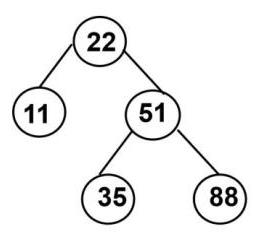
\includegraphics[width=0.3\textwidth]{images/2023/blank_10.jpg}
    \caption*{图1 10题图} % 使用带星号的 caption*
\end{figure}

11. 在有序表 A[1..11]中, 采用折半查找算法查等于 A[8]的元素, 所比较的元素下标依次为\_\_\_\_\_\_\_\_。

12. 已知待排序的 \(n\) 个元素可分为 \(n/k\) 个组,每个组包含 \(k\) 个元素,且任一组内的各元素均分别大于前一组内的所有元素和小于后一组内的所有元素,若采用基于比较的排序,其时间下界为\_\_\_\_\_\_\_\_。

13. 对 \(n\) 个记录的文件进行堆排序,最坏情况下的执行时间下界是\_\_\_\_\_\_\_\_。

14. 在含有 \(n\) 个结点的三叉链表中有\_\_\_\_\_\_\_\_个空链域。

\section*{三. 综合应用题 (本大题共 8 小题, 共 70 分)}

15.(6分)设一个有向图 \(G = \left( {V,E}\right)\) ,其中:

\(V = \left\{  {{v}_{1},{v}_{2},{v}_{3},{v}_{4},{v}_{5}}\right\}  ,\)

\(\left. {E = \left\{  { < {v}_{1},{v}_{5} > , < {v}_{1},{v}_{2} > , < {v}_{1},{v}_{3} > , < {v}_{2},{v}_{3} > , < {v}_{3},{v}_{4} > , < {v}_{5},{v}_{4} > }\right\}  }\right\}\)

给出其所有的拓扑序列。
\vspace{10em}

16. ( 3 分) 画出一个二叉树,使得它既满足大根堆的要求,又满足二叉查找树的要求。

\begin{figure}[htbp]
    \centering
    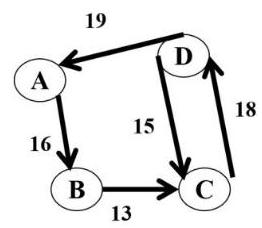
\includegraphics[width=0.3\textwidth]{images/2023/comprehensive_16.jpg}
    \caption*{图2 17题图} % 使用带星号的 caption*
\end{figure}
\vspace{10em}

\newpage
17. (8 分) 一个有向图 \(G\) 如图 2 所示: 使用单源点最短路径算法 Dijkstra 求解图 \(G\) 中 \(\mathrm{A}\) 点到其他各点的最短路径, 要求给出计算过程。
\vspace{10em}

18.(13分)图 3 是一个有三棵树的森林。

(1)采用二叉链表(孩子兄弟表示法)来存储森林,画出该森林对应的二叉树;

(2)画出上述二叉树的后序线索树；

(3)用先序和中序分别遍历该森林,写出遍历后的结点序列。

\begin{figure}[htbp]
    \centering
    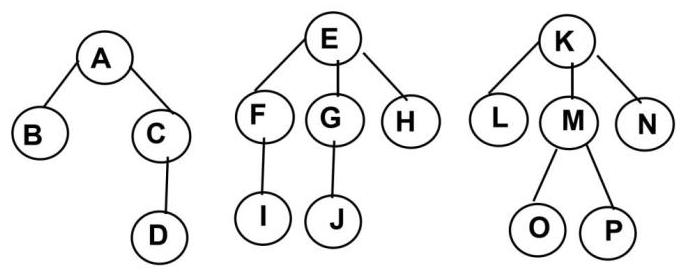
\includegraphics[width=0.3\textwidth]{images/2023/comprehensive_18.jpg}
    \caption*{图3 18题图} % 使用带星号的 caption*
\end{figure}
\vspace{10em}

\newpage
19. (7 分) 设散列表为 \({HT}\left\lbrack  {0.{.9}}\right\rbrack\) ,即表的大小为 \(m = {10}\) 。现采用双散列法解决冲突。散列函数和再哈希函数分别为:

\({h}_{1}\left( x\right)  = x{\;\operatorname{mod}\;{10}},\)

\({h}_{2}\left( x\right)  = 7 - \left( {x{\;\operatorname{mod}\;7}}\right)\) 。

若插入的关键码序列为(4371, 1323, 6173, 4199, 4344, 9679, 1989),写出上述各关键字在表中的位置。(即:填写完整如下所示表格。)

\begin{center}
\begin{tabular}{|c|c|c|c|c|c|c|c|c|c|c|}
\hline
哈希地址 & 0 & 1 & 2 & 3 & 4 & 5 & 6 & 7 & 8 & 9 \\
\cline{1-11}
关键字 & \phantom{X} & \phantom{X} & \phantom{X} & \phantom{X} & \phantom{X} & \phantom{X} & \phantom{X} & \phantom{X} & \phantom{X} & \phantom{X} \\
\cline{1-11}
\hline
\end{tabular}
\end{center}

\vspace{5em}

20. (10分)设某通信信息由 a, b, c, d, e, f 这 6 个字母组成,每个字母出现的次数分别为 5, 9, 12, 13, 16, 45。每个字母在信息传输时需要 1Byte(字节) 的空间。现在将这个信息采用赫夫曼(Huffman)算法压缩成二进制 0,1 序列传输。请问:

(1)压缩后的信息将节约多少 bits(位)？

(2)画出这里设计的 Huffman 树。
\vspace{10em}

\newpage
21. ( 13 分)已知图 G 如图 4 所示:

\begin{figure}[htbp]
    \centering
    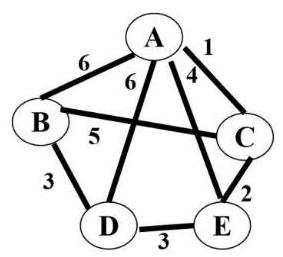
\includegraphics[width=0.3\textwidth]{images/2023/comprehensive_21.jpg}
    \caption*{图4 21题图} % 使用带星号的 caption*
\end{figure}

(1)画出 G 的邻接表表示图；

(2)根据你画的邻接表,以顶点 \(\mathrm{A}\) 为根, 画出 \(G\) 的深度优先生成树;

(3)根据普里姆(Prim)算法,求图 \(\mathrm{G}\) 从顶点 \(\mathrm{A}\) 出发的最小生成树,要求表示出其每一步生成过程。
\vspace{10em}

22. (10分)设一数组中有数据:5,1,4,6,3,8,2,7。写出用下列排序算法进行一遍排序后的结果。

(1) 冒泡排序 (2)直接插入排序 (3) 快速排序

(4) 简单选择排序 (5) 二路归并排序
\vspace{10em}

\section*{四. 算法设计与分析题 (本大题共 2 小题, 共 30 分)}

23. (15分)已知 \(L\) 为链表的头结点地址,表中共有 \(m\left( {m > 3}\right)\) 个结点,从表中第 \(i\left( {1 < i < m}\right)\) 个结点起到第 \(m\) 个结点构成一个循环部分链表。试设计一时间复杂度 \(\mathrm{O}\left( n\right)\) 的算法 PatternInvert \(\mathrm{L}\left( {\text{ LinkList }L\text{ , int }i\text{ , int }m}\right)\) ,将这部分循环链表中所有结点顺序完全倒置。要求:

(1)描述算法的基本设计思想；

(2)根据设计思想,采用 \(\mathrm{C}\) 语言描述算法,关键之处给出注释。

\begin{figure}[htbp]
    \centering
    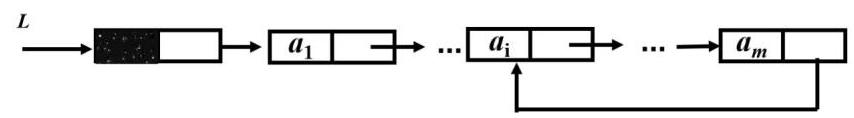
\includegraphics[width=0.3\textwidth]{images/2023/algorithm_23.jpg}
    \caption*{图4 21题图} % 使用带星号的 caption*
\end{figure}

结点定义如下:



typedef struct node

\{

\hspace*{1em} int data;

\hspace*{1em} struct node *next;

\}LNode,*LinkList;
\vspace{13em}

24. (15分)给定一个 \({nm}\) 的矩形位图,位图中的每个像素不是白色就是黑色,但至少有一个是白色的。第 \(i\) 行第 \(j\) 列的像素被称作像素(i, j)。两个像素 \({p}_{1} = \left( {{i}_{1},{j}_{1}}\right) ,{p}_{2} = \left( {{i}_{2},{j}_{2}}\right)\) 之间的距离定义为: \(d\left( {{p}_{1},{p}_{2}}\right)  = \left| {{i}_{1} - {i}_{2}}\right|  + \left| {{j}_{1} - {j}_{2}}\right|\) 。现在请设计一个时间复杂度尽可能低的算法来计算图中每个像素与离其最近的“白像素”的距离。

输入: 第 1 行包含两个整数 \(n\) 和 \(m\left( {1 \leq  n \leq  {150},1 \leq  m \leq  {150}}\right)\) ,用一个空格隔开。 接下来 \(n\) 行,每一行都包含一个长度为 \(m\) 的 01 串。第 \(i + 1\) 行第 \(j\) 列的字符若为 1 ,则像素(i, j)是白色的；否则是黑色的。

输出: 包含 \(n\) 行,每行有 \(m\) 个用空格隔开的整数。第 \(i\) 行第 \(j\) 列的整数表示(i, j)与离其最近的白像素之间的距离。

要求:

(1)描述算法的基本设计思想；

(2)根据设计思想,采用类 \(\mathrm{C}\) 语言的伪代码描述算法,关键之处给出注释。

( 3 )说明你所设计的算法的时间复杂度。
